\documentclass[a4paper, 12pt]{report}

% --- PAQUETS ESSENTIELS ---
\usepackage{wrapfig}
\usepackage[french]{babel}
\usepackage[utf8]{inputenc}
\usepackage[T1]{fontenc}
\usepackage{graphicx}
\usepackage{geometry}
\usepackage{xcolor}
\usepackage{listings}
\usepackage[hidelinks]{hyperref}
\usepackage{float}
\usepackage{amsmath}
\usepackage{fancyhdr}
\usepackage{lastpage}
\usepackage{caption}
\usepackage{subcaption}
\usepackage{verbatim}
\usepackage{listingsutf8}
\usepackage{enumitem}
\usepackage{titlesec}
\usepackage{tikz}
\usepackage{mdframed}
\usepackage{booktabs}
\usepackage{tabularx}

\geometry{
    a4paper,
    left=20mm,
    right=20mm,
    top=25mm,
    bottom=25mm
}

% Fix numérotation : sections en 1, 1.1, 1.1.1 (pas 0.1)
\renewcommand{\thesection}{\arabic{section}}
\renewcommand{\thesubsection}{\thesection.\arabic{subsection}}
\renewcommand{\thesubsubsection}{\thesubsection.\arabic{subsubsection}}

\begin{document}

\begin{titlepage}
    \centering

    \includegraphics[width=0.38\textwidth]{./UdP.jpg}

    \vspace{4cm}

    {\Huge \textbf{Rapport de Projet IA}\par}
    \vspace{0.8cm}
    {\LARGE \textbf{Quoridor --- Minimax Alpha-Bêta}\par}
    \vspace{0.4cm}

    \vspace{2cm}

    {\large
    Membre du projet : \par Danil GUIDJOU\par Anis HAMMOUCHE
    \vspace{0.3cm}

    }

    \vspace{1cm}

    \vfill

    {\large Année universitaire 2025--2026\par}
\end{titlepage}

\tableofcontents
\newpage

\section{Présentation générale du jeu}

Le Quoridor est un jeu de plateau créé par Mirko Marchesi. Deux joueurs s'affrontent sur une grille de 9$\times$9 cases. Chacun contrôle un pion et dispose de 10 murs à poser au fil de la partie. Le joueur 1 démarre au centre de la première ligne (position $(4,0)$), le joueur 2 au centre de la dernière (position $(4,8)$).

\subsection{Règles principales}

À chaque tour, un joueur choisit entre deux actions :
\begin{itemize}
    \item Déplacer son pion d'une case (haut, bas, gauche ou droite), à condition qu'un mur ne bloque pas le passage.
    \item Poser un mur de 2 cases de long, horizontal ou vertical, ce qui consomme un mur de son stock.
\end{itemize}

Quand l'adversaire occupe la case adjacente, on peut le sauter (avancer de 2 cases). Si un mur ou le bord empêche ce saut direct, on saute en diagonale.

\subsection{Conditions de victoire}

\begin{itemize}
    \item Le joueur 1 gagne en atteignant la ligne $y=8$ (bord opposé).
    \item Le joueur 2 gagne en atteignant la ligne $y=0$ (bord opposé).
\end{itemize}

\subsection{Contrainte fondamentale}

On ne peut pas poser un mur s'il coupe tout chemin vers la ligne d'arrivée d'un des deux joueurs. On vérifie ça avec un BFS (parcours en largeur) après chaque tentative de pose.

\subsection{Simplifications retenues}

Les règles sont identiques à la version officielle. On a juste ajouté une limite de 200 coups par partie, pour éviter que les matchs entre IA tournent en boucle.

%------------------------------------------------------------------
\section{Implémentation et validation du moteur de jeu}

\subsection{Représentation de l'état}

Toute la logique du jeu est dans la classe \texttt{QuoridorBoard}. L'état d'une partie tient dans quatre attributs :

\begin{itemize}
    \item \texttt{positions} : dictionnaire $\{1: (x_1, y_1),\ 2: (x_2, y_2)\}$ pour la position de chaque pion.
    \item \texttt{walls} : ensemble de tuples $(x, y, orientation)$ avec $orientation \in \{$\texttt{'H'}, \texttt{'V'}$\}$. Un mur horizontal en $(x,y)$ bloque le passage entre les lignes $y$ et $y+1$ sur les colonnes $x$ et $x+1$.
    \item \texttt{walls\_count} : dictionnaire $\{1: n_1,\ 2: n_2\}$, le nombre de murs restants par joueur.
    \item \texttt{winner} : \texttt{None} tant que la partie continue, sinon l'identifiant du vainqueur.
\end{itemize}

\subsection{Génération des coups légaux}

\texttt{get\_legal\_pawn\_moves(player\_id)} retourne la liste des cases accessibles. La méthode gère les murs, les bords du plateau et les sauts (directs ou diagonaux quand l'adversaire est adjacent). Elle s'appuie sur \texttt{get\_accessible\_neighbors(x, y)} qui donne les voisins non bloqués par un mur.

\subsection{Validation des murs}

\texttt{place\_wall} passe par plusieurs vérifications :
\begin{enumerate}
    \item Le joueur a-t-il encore des murs ? (stock $> 0$)
    \item Les coordonnées sont-elles dans la grille ? ($0 \leq x, y \leq 7$)
    \item Pas de chevauchement avec un mur existant ? (\texttt{\_is\_wall\_placement\_valid})
    \item Les deux joueurs ont-ils toujours un chemin ? (BFS via \texttt{is\_path\_available})
\end{enumerate}

\subsection{Détection des états terminaux}

La victoire est vérifiée dans \texttt{move\_pawn} : dès qu'un pion atteint sa ligne cible, \texttt{winner} est mis à jour et la partie s'arrête.

\subsection{Tests unitaires}

15 tests avec \texttt{pytest} couvrent l'initialisation, la copie du board, les déplacements (cas normal, hors plateau, bloqué par mur), les sauts (direct, diagonal, au bord), la pose de murs (valide, stock épuisé, chevauchements, blocage) et la détection de victoire. Ils passent tous.

%------------------------------------------------------------------
\section{Algorithmes de décision et fonctions d'évaluation}

\subsection{Algorithme Minimax}

On a d'abord implémenté le Minimax classique, sans aucune optimisation de recherche (\texttt{src/ia/minimax.py}). L'idée est simple : on explore l'arbre de jeu jusqu'à une profondeur fixée. À chaque n\oe{}ud, le joueur courant (MAX) choisit le coup qui maximise son score, et l'adversaire (MIN) choisit celui qui le minimise. À la profondeur limite, on évalue la position avec une heuristique.

L'algorithme explore tous les n\oe{}uds sans exception, ce qui donne une complexité en $O(b^d)$ avec $b$ le facteur de branchement et $d$ la profondeur. 
%C'est conforme à la définition de Russell \& Norvig (\textit{AI: A Modern Approach}).

\texttt{get\_best\_move} appelle le minimax sur chaque coup possible et garde le meilleur. On a aussi ajouté un mécanisme anti-oscillation : l'IA garde en mémoire ses 6 dernières positions, et pénalise de $-50$ tout retour sur une case récente. Sans ça, les IA D1 font des aller-retours sans fin.

\subsection{Élagage alpha-bêta}

Le Minimax pur explore beaucoup de branches inutiles. Si on sait déjà qu'un coup donne un score de 10, pourquoi continuer à explorer une branche où l'adversaire peut nous forcer en dessous ? C'est le principe de l'élagage alpha-bêta (\texttt{src/ia/elagage.py}).

On maintient deux bornes : $\alpha$ (le meilleur score garanti pour MAX) et $\beta$ (le meilleur score garanti pour MIN). Dès que $\alpha \geq \beta$, on coupe la branche. Dans le cas optimal, ça réduit la complexité de $O(b^d)$ à $O(b^{d/2})$. En pratique, ça veut dire que l'élagage à profondeur 4 explore à peu près autant de n\oe{}uds que le Minimax pur à profondeur 2.

L'$\alpha$ de la racine est mis à jour avec le score brut, pas le score pénalisé par l'anti-oscillation. Sinon l'élagage serait faussé.

\subsection{Optimisation du facteur de branchement}

Le Quoridor a un facteur de branchement d'environ 72 (4-5 déplacements + $\sim$67 murs possibles). Trop pour chercher en profondeur, même avec élagage. Le module \texttt{moves\_optimization.py} ramène ça à 10--15 coups :
\begin{enumerate}
    \item Les déplacements de pion en premier, triés par progression vers l'objectif.
    \item Pour les murs, seuls ceux dans une zone autour des deux joueurs (marge de 2 cases) sont considérés.
    \item Chaque mur candidat est simulé via BFS : on ne garde que ceux qui gênent plus l'adversaire que nous ($gain_{adv} \geq cost_{self}$ et $gain_{adv} > 0$).
    \item Les murs restants sont triés par gain net décroissant, pour que l'élagage coupe vite.
\end{enumerate}

Mertens (2006) était limité à la profondeur 2 avec un facteur de branchement de 60--70. Notre filtrage permet d'atteindre D3 et D4.

\subsection{Trois fonctions d'évaluation}

\subsubsection{Heuristique simple (\texttt{heuristic\_simple\_distance})}

\begin{equation}
    score = (dist_{adv} - dist_{joueur}) \times 10
\end{equation}

On compare la distance BFS de chaque joueur vers sa ligne d'arrivée. Plus l'adversaire est loin et plus on est proche, mieux c'est.

\subsubsection{Heuristique avancée (\texttt{heuristic\_shortest\_path})}

\begin{equation}
    score = (dist_{adv} - dist_{joueur}) \times 10 + (murs_{joueur} - murs_{adv}) \times 5
\end{equation}

Même base, mais on valorise aussi le fait d'avoir gardé ses murs. Un joueur qui a des murs en réserve peut encore bloquer l'adversaire.

\subsubsection{Heuristique experte (\texttt{heuristic\_expert})}

\begin{equation}
    score = (dist_{adv} - dist_{joueur}) \times 10 + \Delta_{murs} \times 5 + progression \times 3 + bonus_{tempo} + bonus_{endgame}
\end{equation}

\begin{itemize}
    \item $progression$ : combien le pion a avancé vers son objectif ($y$ pour J1, $8-y$ pour J2). Ça pousse à avancer au lieu de stagner.
    \item $bonus_{tempo}$ : quand on mène la course et qu'on a des murs pour se défendre, le score est amplifié ($+\Delta_{dist} \times 3$).
    \item $bonus_{endgame}$ : si l'adversaire n'a plus de murs, il ne peut pas nous bloquer donc on essaye d'aller tout droit.
\end{itemize}

\subsection{Analyse expérimentale}

Le tableau~\ref{tab:perf} résume les performances en poules (9 matchs par IA).

\begin{table}[H]
\centering
\caption{Performances en poules par configuration (sur 9 matchs par IA)}
\label{tab:perf}
\begin{tabular}{llccc}
\toprule
\textbf{IA} & \textbf{Config} & \textbf{Victoires} & \textbf{Défaites} & \textbf{Temps moy. (s)} \\
\midrule
Naive & D1, simple & 2 & 7 & 0.3 \\
Agressive & D1, expert & 3 & 6 & 0.2 \\
Prudente & D1, advanced & 2 & 7 & 0.2 \\
Calculatrice & D2, simple & 4 & 5 & 2.3 \\
Stratège & D2, advanced & 4 & 5 & 2.1 \\
Commandante & D2, expert & 5 & 4 & 1.9 \\
Visionnaire & D3, advanced & 6 & 3 & 18.5 \\
Maîtresse & D3, expert & 7 & 2 & 19.2 \\
\bottomrule
\end{tabular}
\end{table}

La profondeur compte le plus. Les IA D3 gagnent la majorité de leurs matchs. À profondeur égale, expert bat advanced, qui bat simple.

Le temps monte vite : 0.2s par coup à D1, 2s à D2, presque 20s à D3. Chercher plus loin donne de meilleures décisions, mais ça se paye.

\subsection{Ordonnancement des coups et élagage}

L'ordre dans lequel on explore les coups a un vrai impact sur l'élagage. En testant les déplacements d'abord (triés par progression) puis les murs par gain décroissant, on tombe vite sur de bons coups. La fenêtre $[\alpha, \beta]$ se resserre et on coupe plus de branches.

On a aussi vu que l'heuristique experte aide l'élagage à couper plus tôt, parce qu'elle différencie mieux les positions. C'est probablement pour ça que la Commandante (D2, expert) bat la Visionnaire (D3, advanced) malgré une profondeur inférieure : elle explore mieux avec moins.

%------------------------------------------------------------------
\section{Tournoi entre les intelligences artificielles}

\subsection{Organisation générale}

On a mis en place deux tournois distincts avec la même structure mais des algorithmes différents :
\begin{itemize}
    \item Tournoi Minimax pur : sans élagage (\texttt{src/ia/minimax.py})
    \item Tournoi Alpha-Bêta : avec élagage alpha-bêta (\texttt{src/ia/elagage.py})
\end{itemize}

Chaque tournoi oppose 12 IA, toutes les combinaisons de profondeur (D1 à D4) et d'heuristique (simple, advanced, expert) :

\begin{table}[H]
\centering
\caption{Les 12 instances du tournoi}
\label{tab:participants}
\begin{tabular}{lcc}
\toprule
\textbf{Nom} & \textbf{Profondeur} & \textbf{Stratégie} \\
\midrule
D1-Simple & 1 & simple \\
D1-Advanced & 1 & advanced \\
D1-Expert & 1 & expert \\
D2-Simple & 2 & simple \\
D2-Advanced & 2 & advanced \\
D2-Expert & 2 & expert \\
D3-Simple & 3 & simple \\
D3-Advanced & 3 & advanced \\
D3-Expert & 3 & expert \\
D4-Simple & 4 & simple \\
D4-Advanced & 4 & advanced \\
D4-Expert & 4 & expert \\
\bottomrule
\end{tabular}
\end{table}

\subsection{Déroulement du tournoi}

Le tournoi se déroule en deux phases.

\subsubsection{Phase de poules}

Les 12 IA sont réparties dans 3 poules de 4, en mélangeant les profondeurs pour éviter de regrouper toutes les IA fortes :

\begin{itemize}
    \item Poule A : D1-Simple, D2-Expert, D3-Advanced, D4-Simple
    \item Poule B : D1-Advanced, D2-Simple, D3-Expert, D4-Advanced
    \item Poule C : D1-Expert, D2-Advanced, D3-Simple, D4-Expert
\end{itemize}

Chaque paire joue 3 matchs avec alternance J1/J2. Ça donne 6 paires $\times$ 3 matchs = 18 matchs par poule, soit 54 matchs en poules.

L'alternance J1/J2 compte parce que le premier joueur a un léger avantage. Trois matchs par paire permettent de le compenser.

Le classement se fait au nombre de victoires. En cas d'égalité, l'ordre de déclaration est conservé.

\subsubsection{Phase éliminatoire}

Les 8 meilleurs passent en élimination directe :
\begin{itemize}
    \item Les 2 premiers de chaque poule (6 qualifiés directs)
    \item Les 2 meilleurs 3\textsuperscript{èmes}
\end{itemize}

La suite se joue en matchs aller-retour (pour alterner le joueur qui commence la partie) :
\begin{enumerate}
    \item Quarts de finale : 4 matchs avec croisements inter-poules
    \item Demi-finales : les 4 vainqueurs
    \item Petite finale : les 2 perdants des demies pour la 3\textsuperscript{ème} place
    \item Grande finale : les 2 vainqueurs pour le titre
\end{enumerate}

Si c'est 1-1, on départage par :
\begin{enumerate}
    \item Le nombre de coups du match gagné (le plus court l'emporte)
    \item Le nombre de murs restants du vainqueur
    \item Un 3\textsuperscript{ème} match avec ordre J1/J2 tiré au sort
\end{enumerate}

Au total, la phase éliminatoire fait environ 16 matchs, pour un total d'environ 70 matchs par tournoi.

%------------------------------------------------------------------
\subsection{Tournoi Minimax pur }

Ce tournoi utilise le Minimax pur. Chaque n\oe{}ud de l'arbre est exploré sans aucune coupure. Complexité : $O(b^d)$ avec $b \approx 12$ après filtrage.

Pour éviter des matchs redondants, on a implémenté un tie-breaking : quand deux coups ont le même score, il y a 20\% de chance de changer de coup. On l'a ensuite retiré car ça introduisait des incohérences où une IA de profondeur 4 perdait face à une IA de profondeur 1.


Durée du tournoi : environ 2 heures, à cause des IA D4 qui explorent l'arbre en entier.

\subsubsection{Résultats}

On a exécuté le tournoi deux fois : une première fois avec tie-breaking (20\% d'aléatoire), puis une seconde fois sans tie-breaking. Le tableau~\ref{tab:classement-minimax} compare les deux classements côte à côte.

\begin{table}[H]
\centering
\caption{Classement Minimax pur : avec vs sans tie-breaking}
\label{tab:classement-minimax}
\begin{tabular}{c|lcc|lcc}
\toprule
\textbf{Rang} & \multicolumn{3}{c|}{\textbf{Avec tie-breaking}} & \multicolumn{3}{c}{\textbf{Sans tie-breaking}} \\
& \textbf{IA} & \textbf{D} & \textbf{Strat.} & \textbf{IA} & \textbf{D} & \textbf{Strat.} \\
\midrule
1 & D2-Expert & 2 & expert & D4-Advanced & 4 & advanced \\
2 & D4-Expert & 4 & expert & D2-Expert & 2 & expert \\
3 & D3-Expert & 3 & expert & D2-Simple & 2 & simple \\
4 & D2-Advanced & 2 & advanced & D4-Simple & 4 & simple \\
5 & D4-Simple & 4 & simple & D3-Expert & 3 & expert \\
6 & D4-Advanced & 4 & advanced & D4-Expert & 4 & expert \\
7 & D3-Simple & 3 & simple & D2-Advanced & 2 & advanced \\
8 & D3-Advanced & 3 & advanced & D3-Advanced & 3 & advanced \\
9 & D2-Simple & 2 & simple & D3-Simple & 3 & simple \\
10 & D1-Simple & 1 & simple & D1-Simple & 1 & simple \\
11 & D1-Advanced & 1 & advanced & D1-Advanced & 1 & advanced \\
12 & D1-Expert & 1 & expert & D1-Expert & 1 & expert \\
\bottomrule
\end{tabular}
\end{table}

\subsubsection{Analyse des résultats}

Avec le tie-breaking, l'heuristique expert occupe le podium en entier (D2, D4, D3). Mais D2-Expert finit premier, devant D4-Expert. C'est une anomalie : une IA de profondeur 2 ne devrait pas battre une de profondeur 4 avec la même heuristique. Le tie-breaking en est la cause --- à D4, l'IA évalue plus de coups à la racine et tombe plus souvent sur des scores égaux, ce qui augmente les chances de dévier du meilleur coup.

Sans le tie-breaking, le classement change beaucoup. D4-Advanced passe en tête, et les résultats sont plus variés en termes d'heuristiques. On remarque que D2-Expert et D2-Simple montent au podium, ce qui montre qu'à profondeur 2 l'algorithme est assez stable pour bien jouer sans aléatoire. D4 ne domine pas autant qu'on pourrait l'espérer : D4-Advanced est premier mais D4-Expert n'est que 6\textsuperscript{ème} et D4-Simple 4\textsuperscript{ème}.

Dans les deux cas, les IA D1 finissent en bas du classement (rangs 10--12). La profondeur 1 ne suffit pas, avec ou sans tie-breaking.

\subsubsection{Graphiques d'analyse}
\begin{figure}[H]
    \centering
    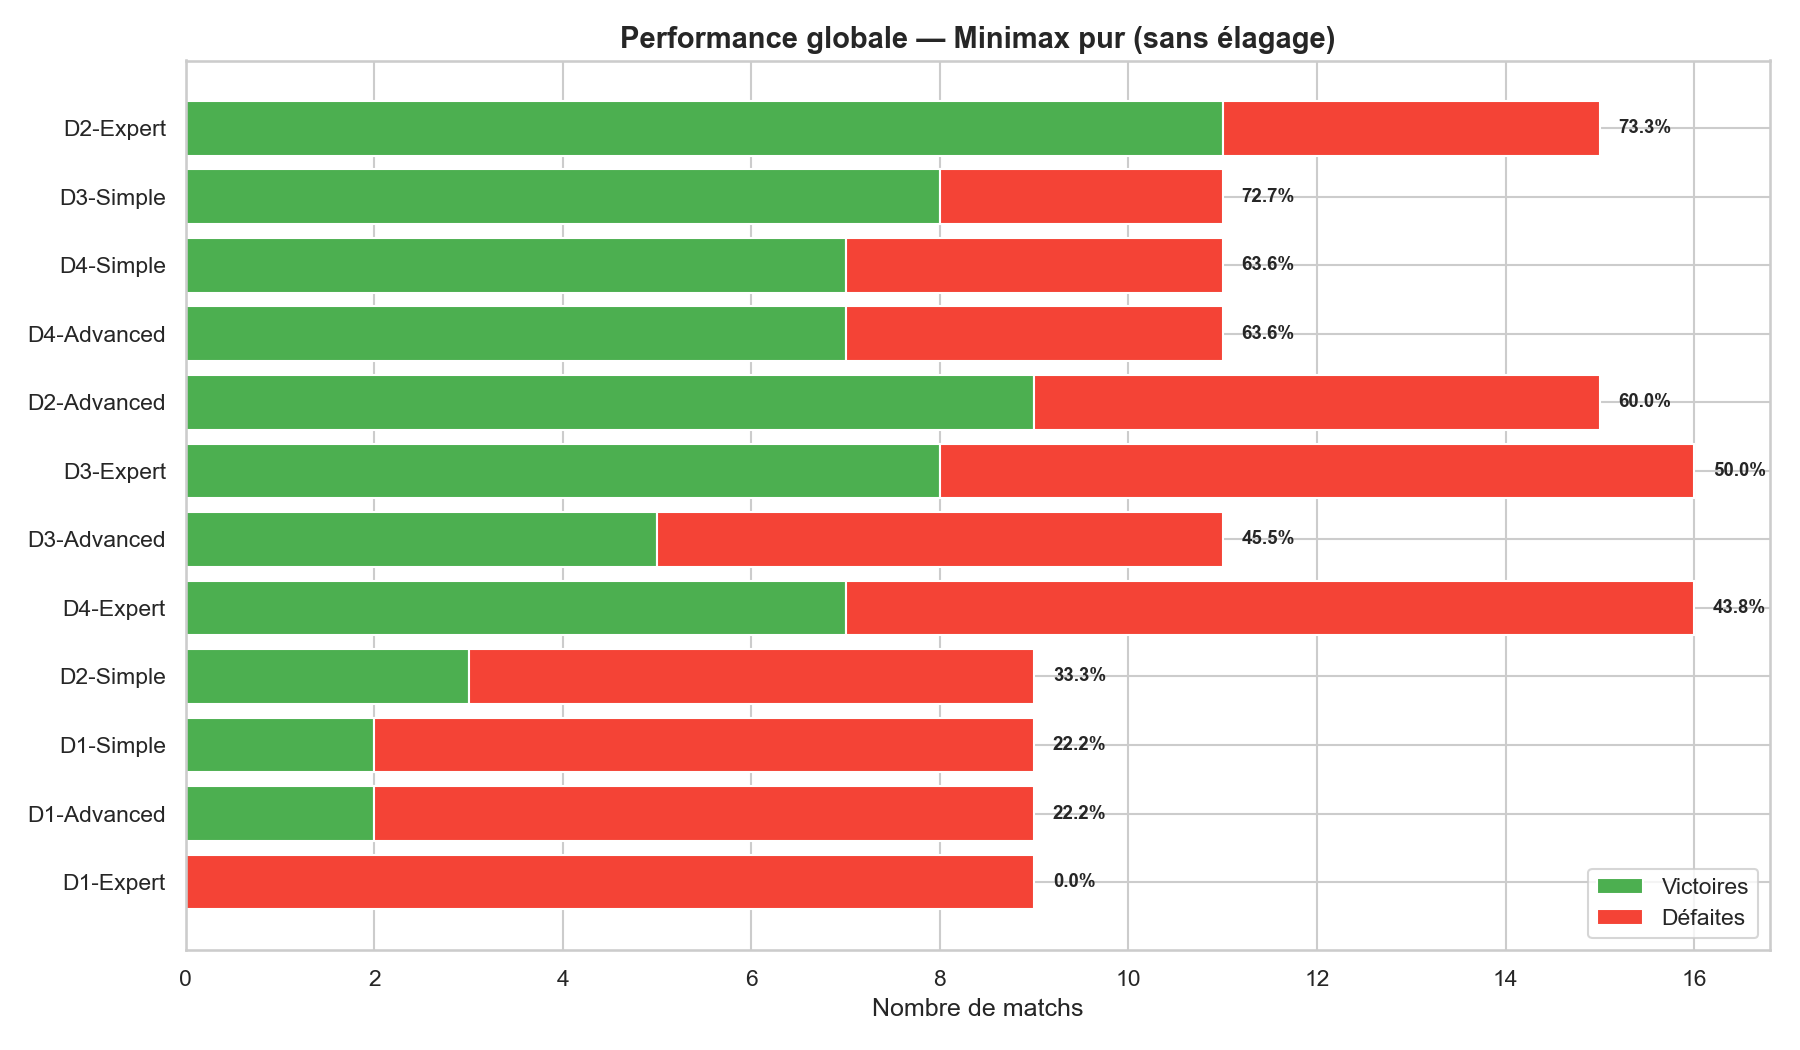
\includegraphics[width=0.85\textwidth]{../data/minimaxRandom/plots/performance_globale.png}
    \caption{Victoires et défaites --- Minimax pur (avec tie-breaking)}
    \label{fig:perf-minimax}
\end{figure}

\begin{figure}[H]
    \centering
    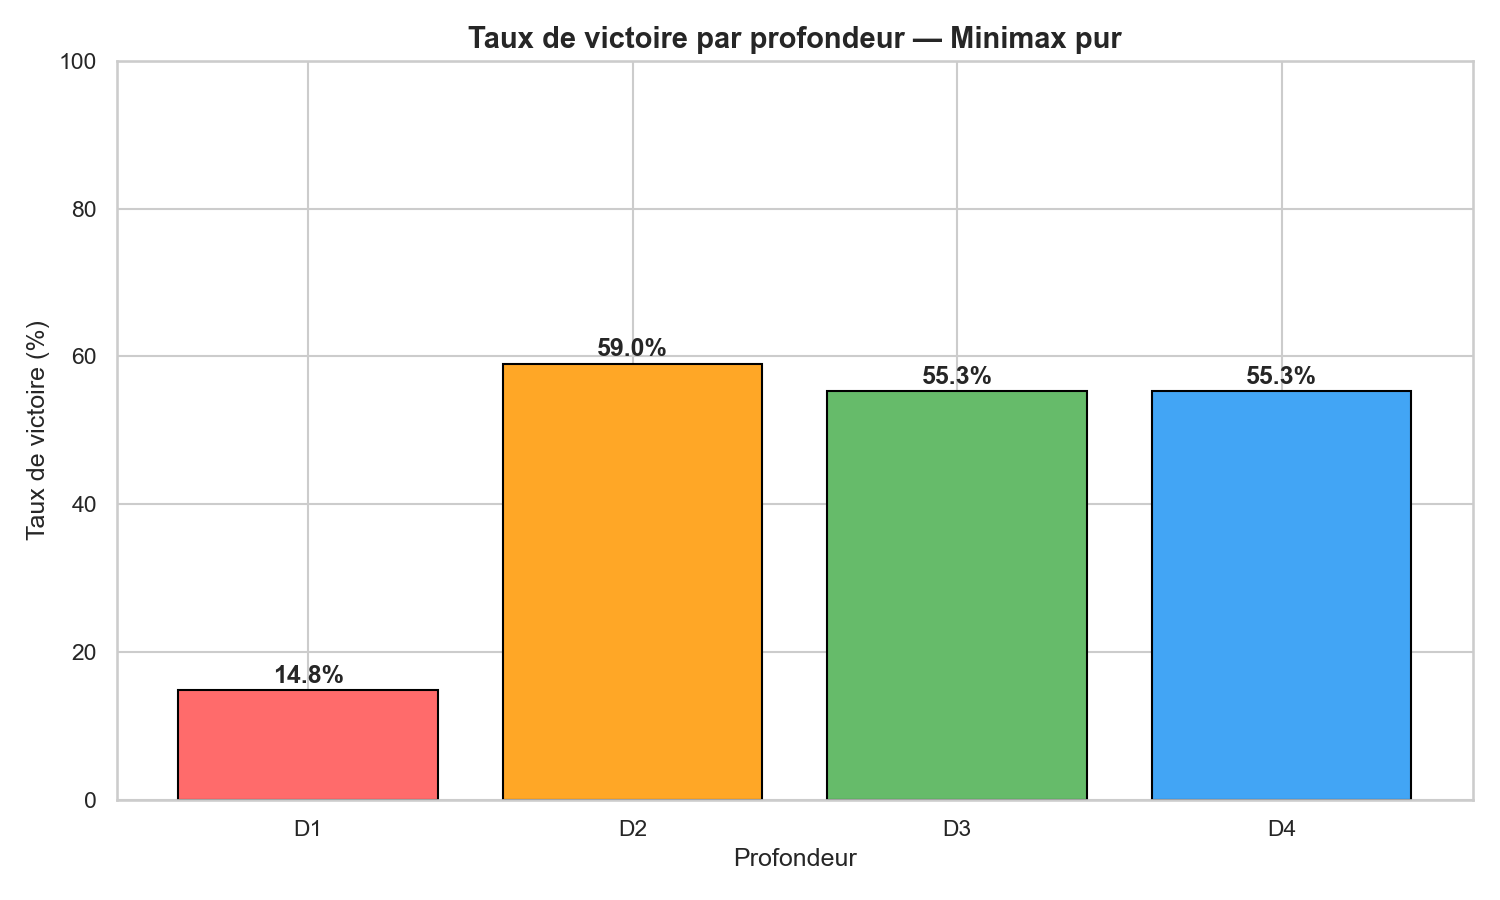
\includegraphics[width=0.85\textwidth]{../data/minimaxRandom/plots/victoires_par_profondeur.png}
    \caption{Taux de victoire par profondeur --- Minimax pur (avec tie-breaking)}
    \label{fig:depth-minimax}
\end{figure}

\begin{figure}[H]
    \centering
    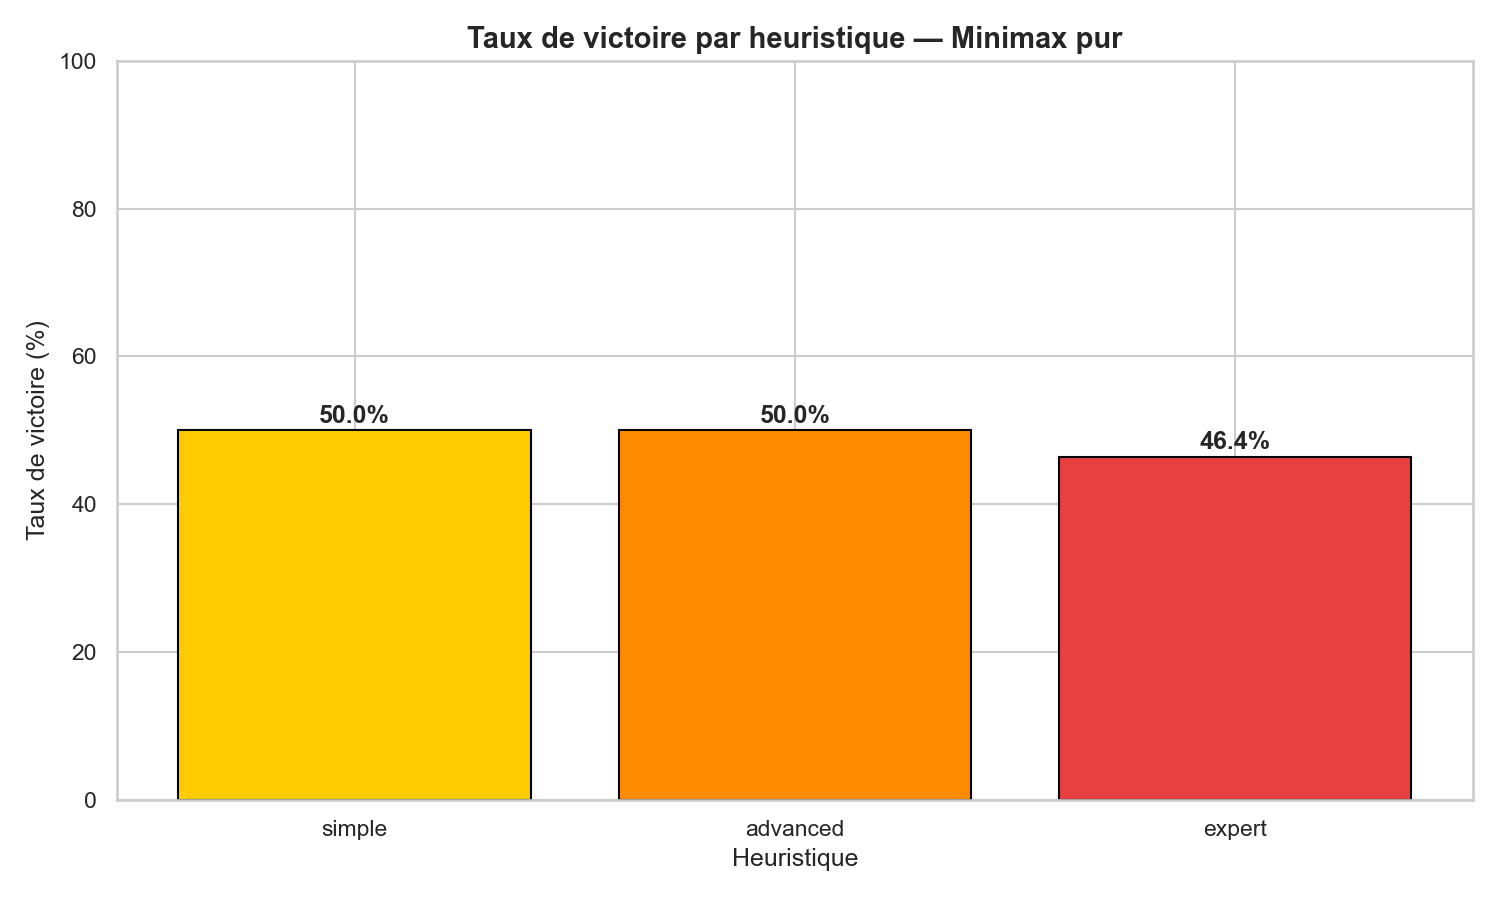
\includegraphics[width=0.85\textwidth]{../data/minimaxRandom/plots/victoires_par_heuristique.png}
    \caption{Taux de victoire par heuristique --- Minimax pur (avec tie-breaking)}
    \label{fig:strat-minimax}
\end{figure}

\begin{figure}[H]
    \centering
    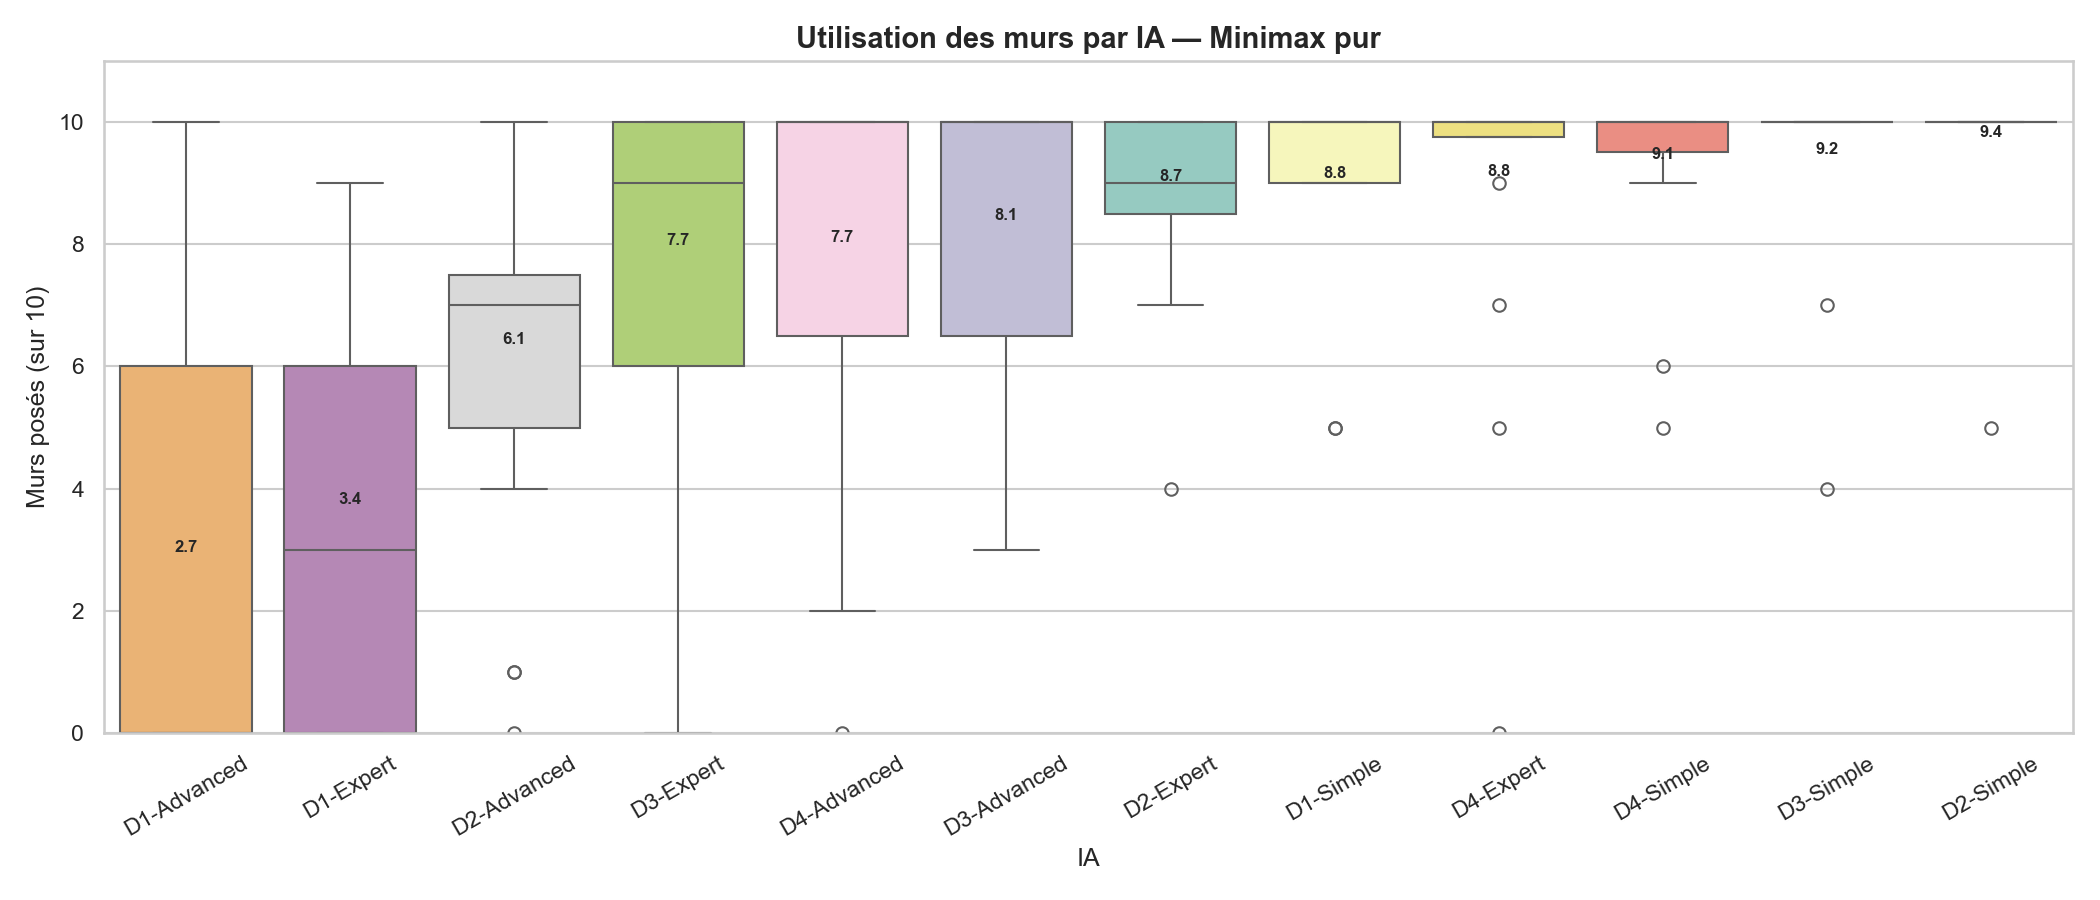
\includegraphics[width=0.85\textwidth]{../data/minimaxRandom/plots/murs_par_ia.png}
    \caption{Utilisation des murs --- Minimax pur (avec tie-breaking)}
    \label{fig:murs-minimax}
\end{figure}

\subsubsection{Graphiques sans tie-breaking}

\begin{figure}[H]
    \centering
    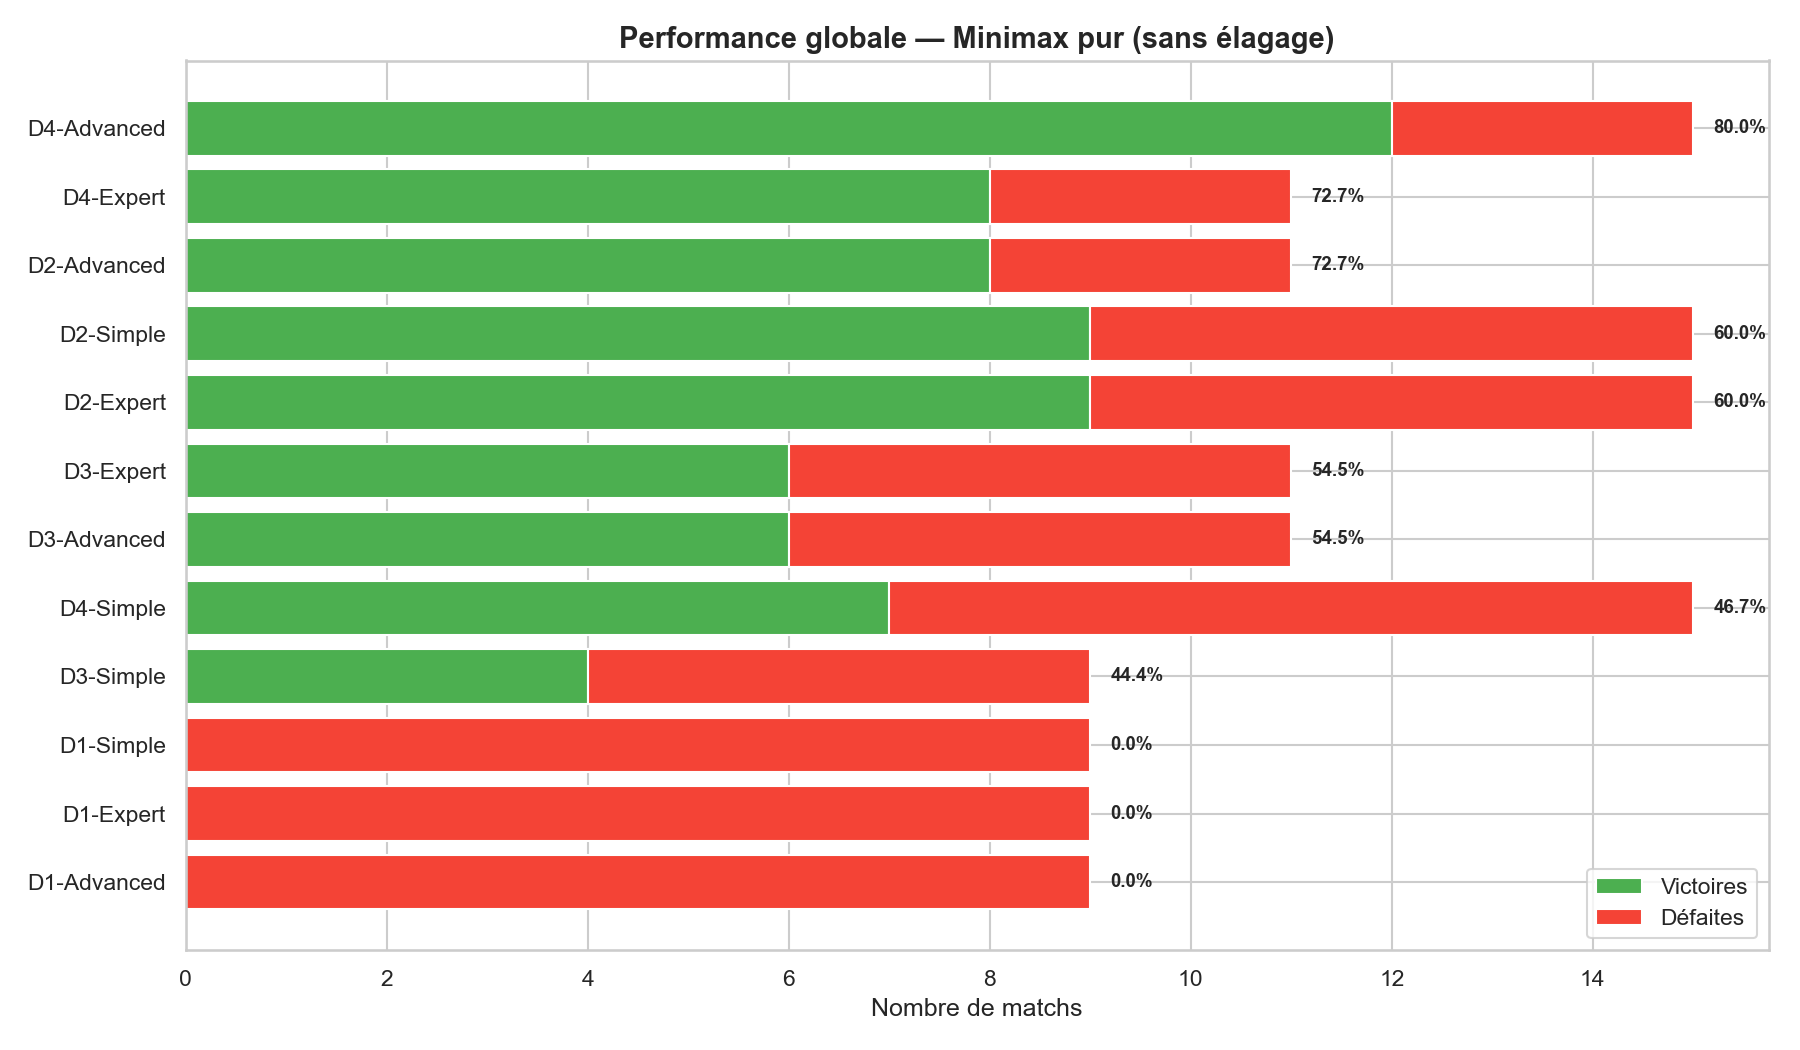
\includegraphics[width=0.85\textwidth]{../data/minimax/plots/performance_globale.png}
    \caption{Victoires et défaites --- Minimax pur (sans tie-breaking)}
    \label{fig:perf-minimax-det}
\end{figure}

\begin{figure}[H]
    \centering
    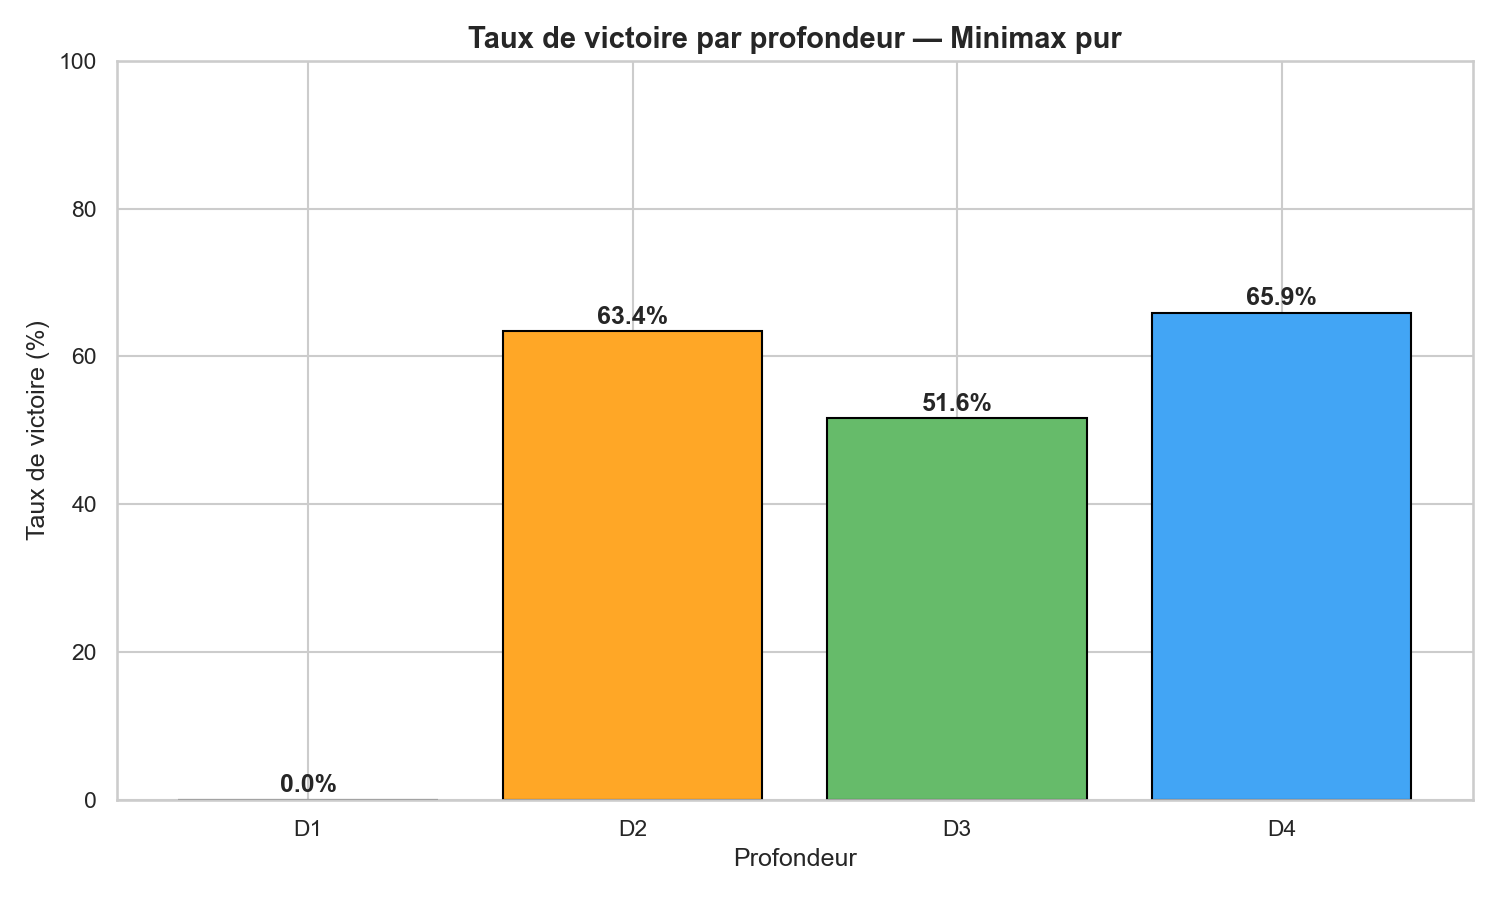
\includegraphics[width=0.85\textwidth]{../data/minimax/plots/victoires_par_profondeur.png}
    \caption{Taux de victoire par profondeur --- Minimax pur (sans tie-breaking)}
    \label{fig:depth-minimax-det}
\end{figure}

\begin{figure}[H]
    \centering
    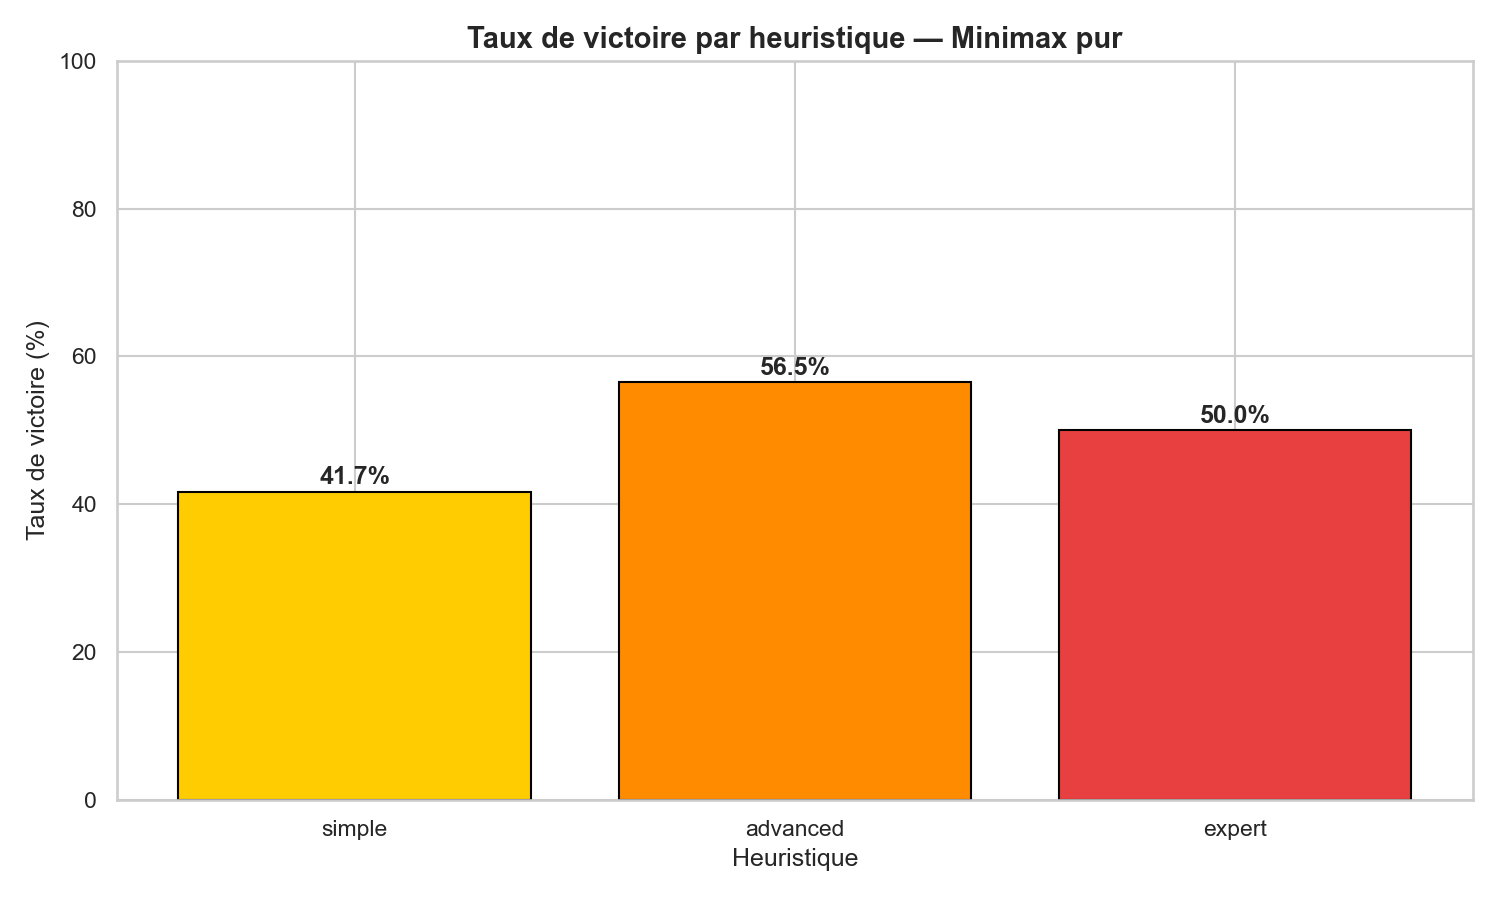
\includegraphics[width=0.85\textwidth]{../data/minimax/plots/victoires_par_heuristique.png}
    \caption{Taux de victoire par heuristique --- Minimax pur (sans tie-breaking)}
    \label{fig:strat-minimax-det}
\end{figure}

\begin{figure}[H]
    \centering
    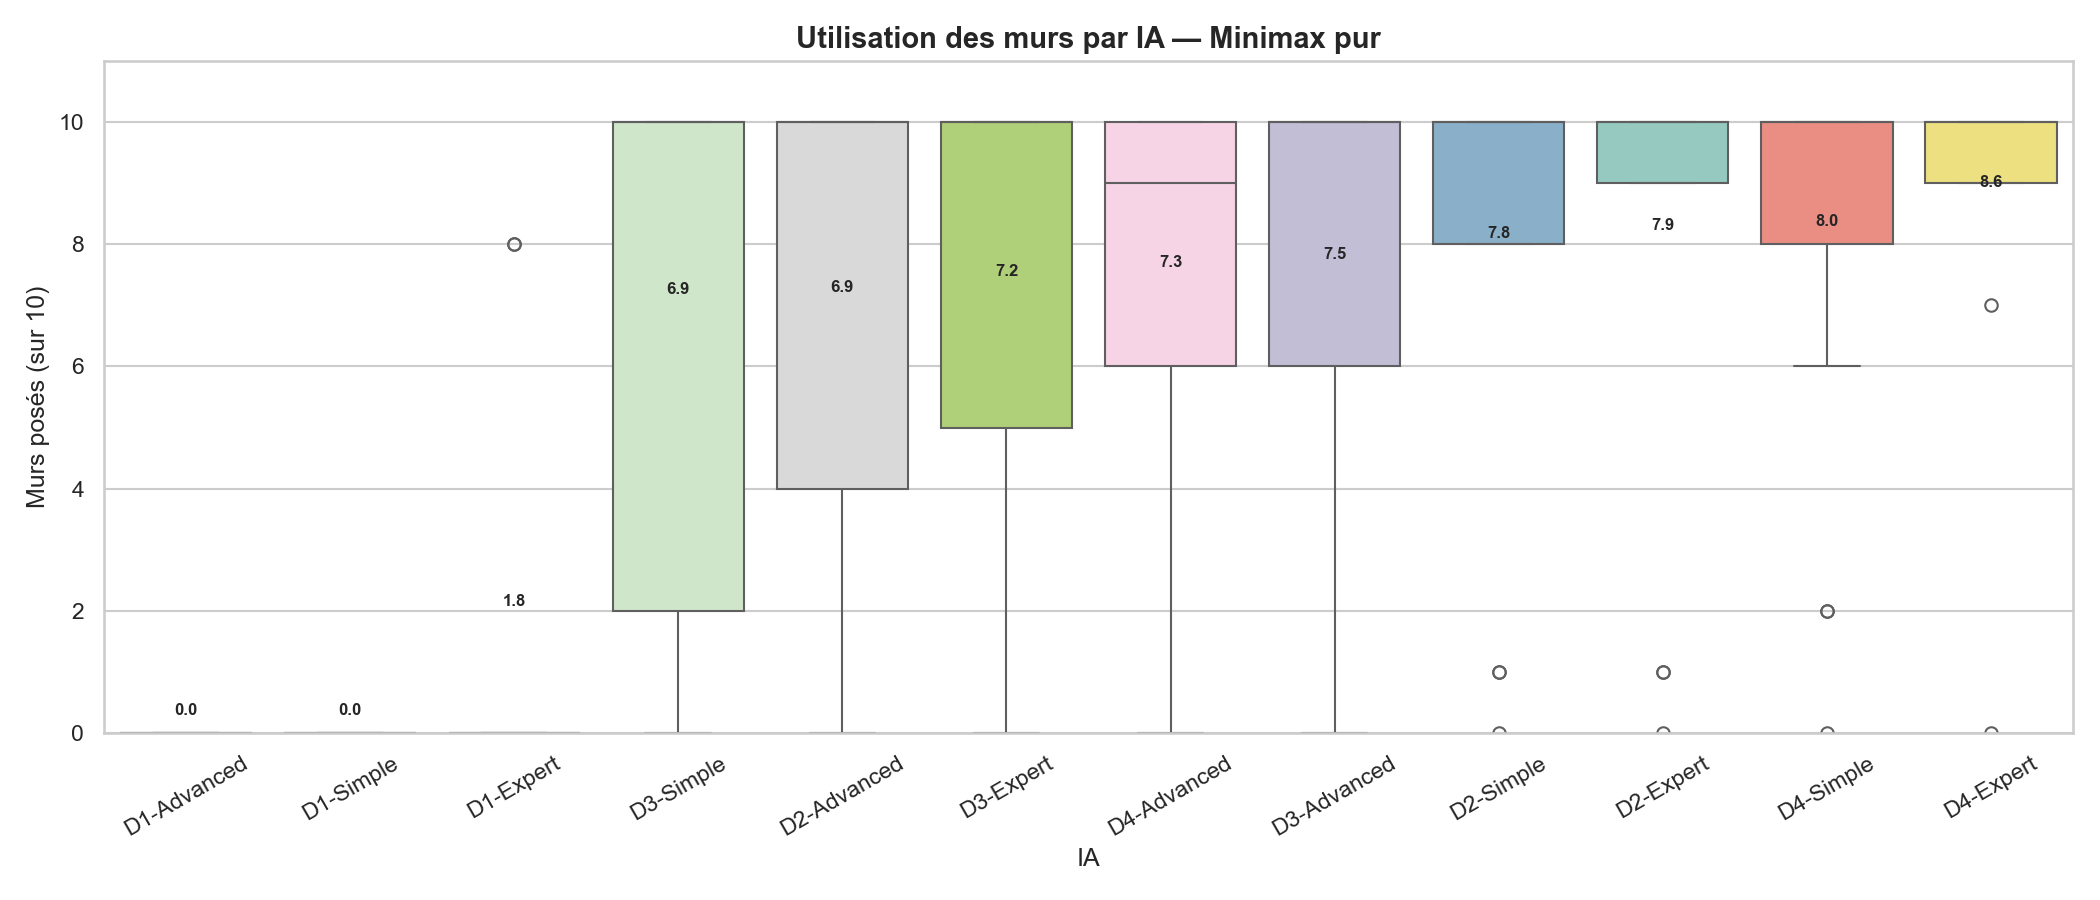
\includegraphics[width=0.85\textwidth]{../data/minimax/plots/murs_par_ia.png}
    \caption{Utilisation des murs --- Minimax pur (sans tie-breaking)}
    \label{fig:murs-minimax-det}
\end{figure}



%------------------------------------------------------------------
\subsection{Tournoi avec élagage alpha-bêta}

Même structure, mais l'algorithme utilise l'élagage alpha-bêta (\texttt{src/ia/elagage.py}). Les branches inutiles sont coupées, ce qui réduit la complexité de $O(b^d)$ à $O(b^{d/2})$ dans le cas optimal. En pratique, l'élagage à D4 explore à peu près autant de n\oe{}uds que le Minimax pur à D2.

Ce tournoi n'utilise aucun tie-breaking aléatoire : à score égal, le premier coup trouvé est conservé. Les résultats sont donc reproductibles.

Durée du tournoi : environ 20 minutes. Beaucoup plus rapide grâce aux coupures.

\subsubsection{Résultats}

\begin{table}[H]
\centering
\caption{Classement final --- Alpha-Bêta}
\label{tab:classement-elagage}
\begin{tabular}{clcc}
\toprule
\textbf{Rang} & \textbf{IA} & \textbf{Profondeur} & \textbf{Stratégie} \\
\midrule
1 & D4-Advanced & 4 & advanced \\
2 & D2-Advanced & 2 & advanced \\
3 & D3-Advanced & 3 & advanced \\
4 & D4-Simple & 4 & simple \\
5 & D2-Simple & 2 & simple \\
6 & D4-Expert & 4 & expert \\
7 & D3-Expert & 3 & expert \\
8 & D2-Expert & 2 & expert \\
9 & D3-Simple & 3 & simple \\
10 & D1-Simple & 1 & simple \\
11 & D1-Advanced & 1 & advanced \\
12 & D1-Expert & 1 & expert \\
\bottomrule
\end{tabular}
\end{table}

\subsubsection{Analyse des résultats}

Cette fois, c'est l'heuristique advanced qui occupe le podium (D4, D2, D3). On ne s'y attendait pas : l'expert, avec ses 5 composantes, devrait en théorie évaluer mieux. Mais l'élagage change la donne.

L'explication : l'heuristique expert produit des scores plus dispersés (5 termes additifs), ce qui rend les coupures moins prévisibles. L'élagage peut couper une branche qui, avec des scores plus homogènes, aurait été explorée et aurait mené au meilleur coup. L'advanced, avec seulement 2 termes (distance + murs), produit des évaluations plus stables et guide l'élagage de manière plus fiable.

La profondeur reste le facteur principal. D4-Advanced bat D3-Advanced, D4-Simple bat D2-Simple. À heuristique égale, chercher plus loin donne toujours un avantage.

D2-Advanced qui atteint la finale est un résultat qui mérite attention. Une IA de profondeur 2 qui rivalise avec D4, c'est possible parce que l'élagage rend D2 très rapide ($\sim$1s/coup) et l'heuristique advanced guide bien les coupures.

Deux matchs se sont terminés en nul (200 coups) en demi-finale, entre des IA de niveau très proche. L'anti-oscillation empêche les boucles courtes (6 dernières positions), mais des cycles plus longs passent à travers.

Les IA D1 sont toutes éliminées en poules (rangs 10--12), comme dans le tournoi Minimax.

\subsubsection{Graphiques d'analyse}

\begin{figure}[H]
    \centering
    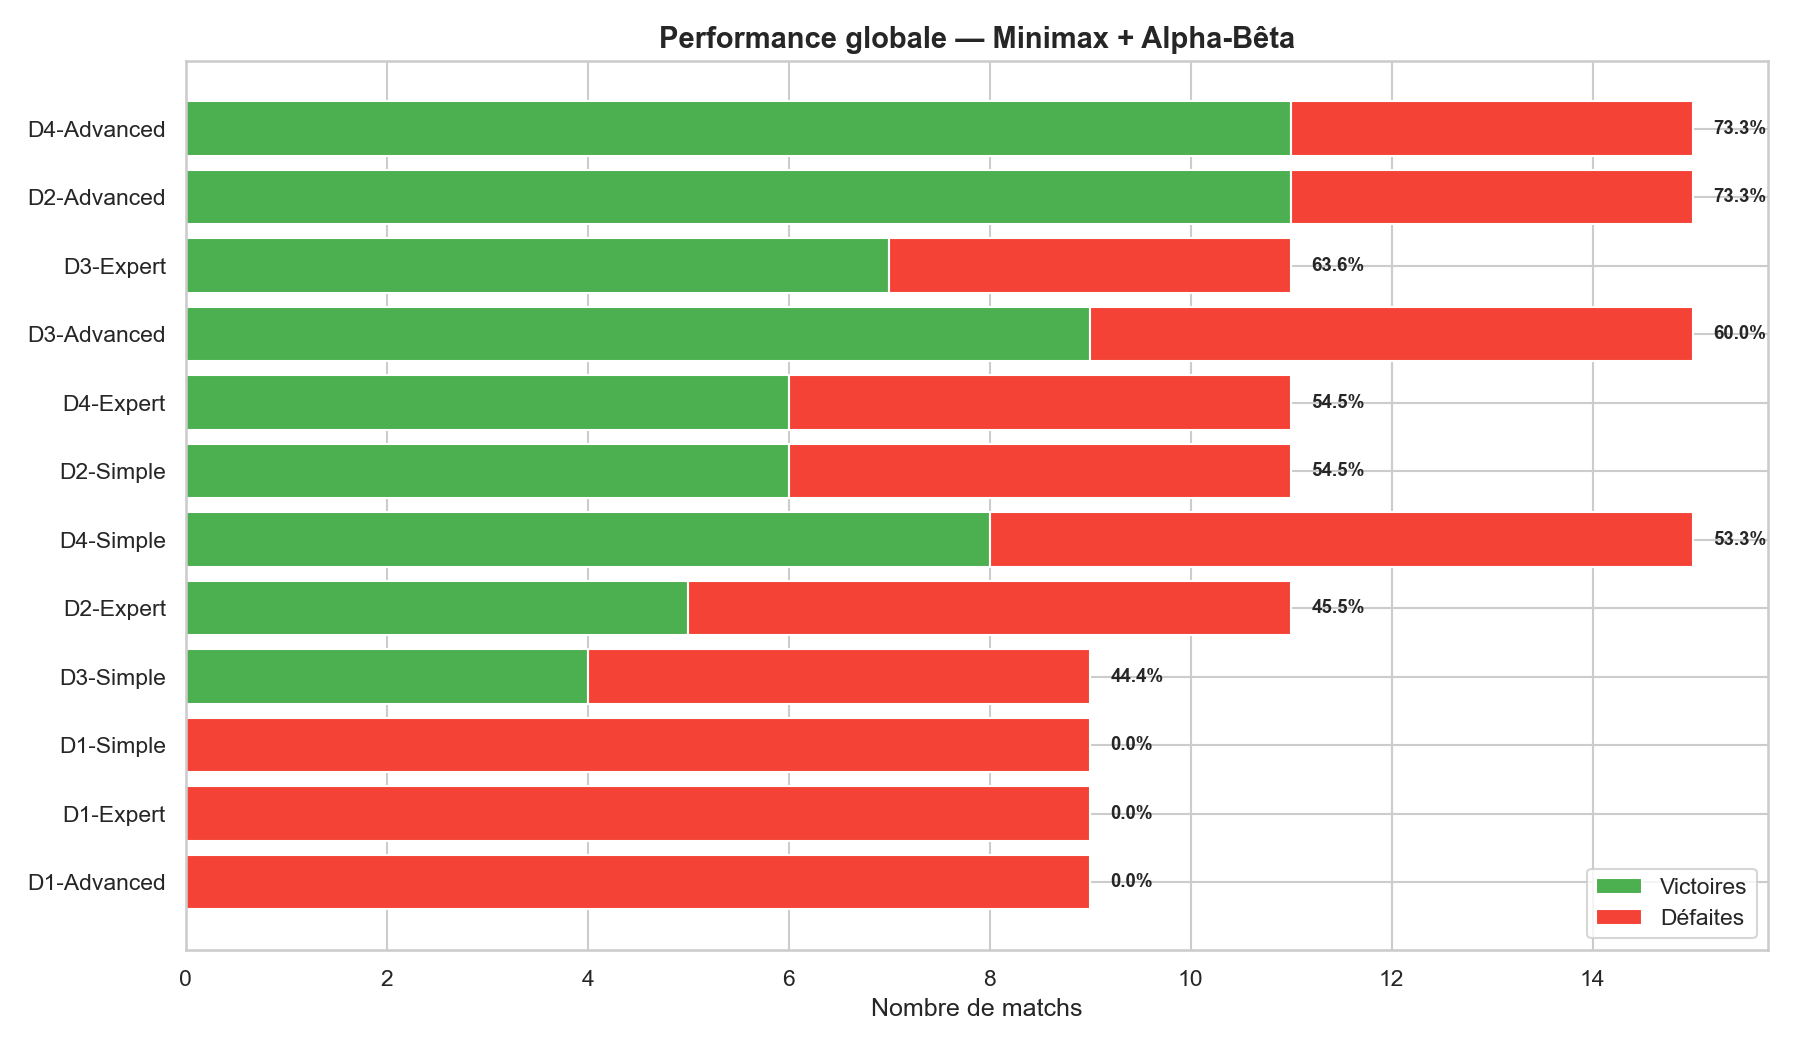
\includegraphics[width=0.85\textwidth]{../data/elagage/plots/performance_globale.png}
    \caption{Victoires et défaites --- Alpha-Bêta}
    \label{fig:perf-elagage}
\end{figure}

\begin{figure}[H]
    \centering
    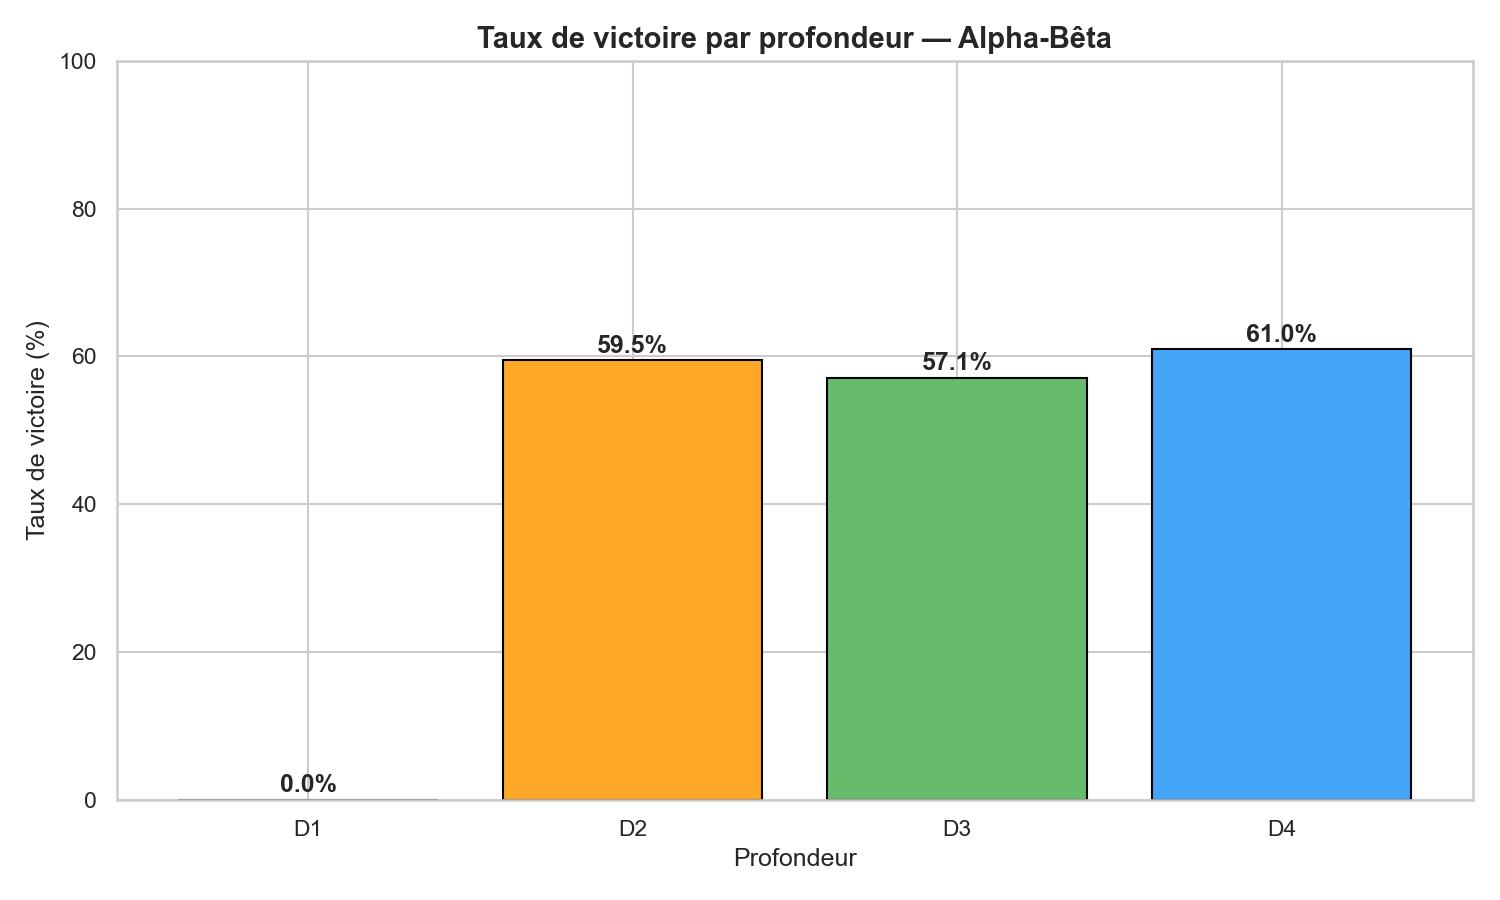
\includegraphics[width=0.85\textwidth]{../data/elagage/plots/victoires_par_profondeur.png}
    \caption{Taux de victoire par profondeur --- Alpha-Bêta}
    \label{fig:depth-elagage}
\end{figure}

\begin{figure}[H]
    \centering
    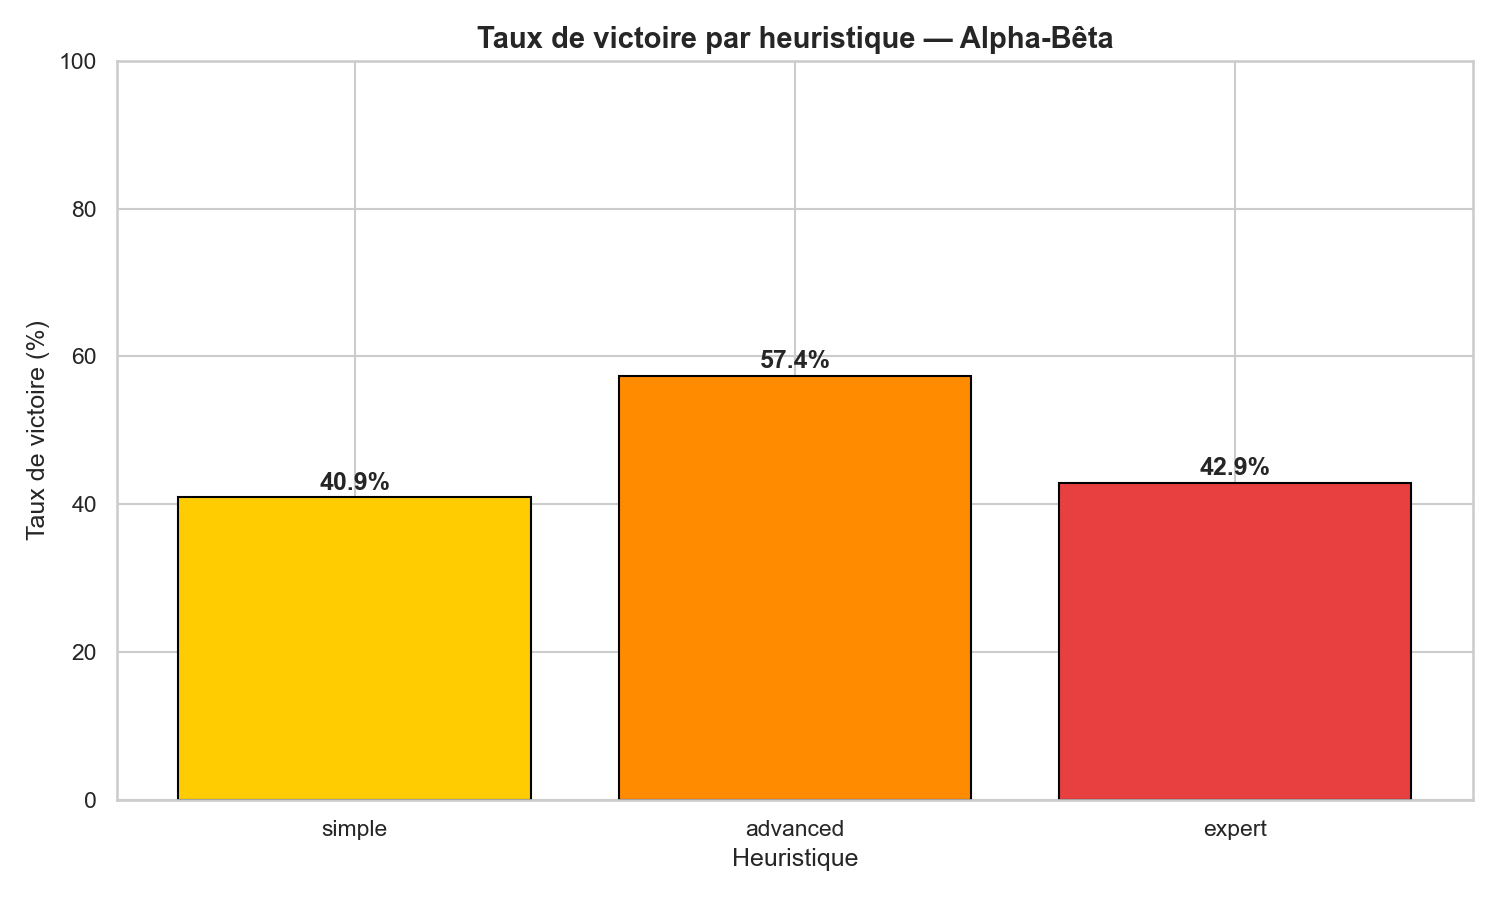
\includegraphics[width=0.85\textwidth]{../data/elagage/plots/victoires_par_heuristique.png}
    \caption{Taux de victoire par heuristique --- Alpha-Bêta}
    \label{fig:strat-elagage}
\end{figure}


\begin{figure}[H]
    \centering
    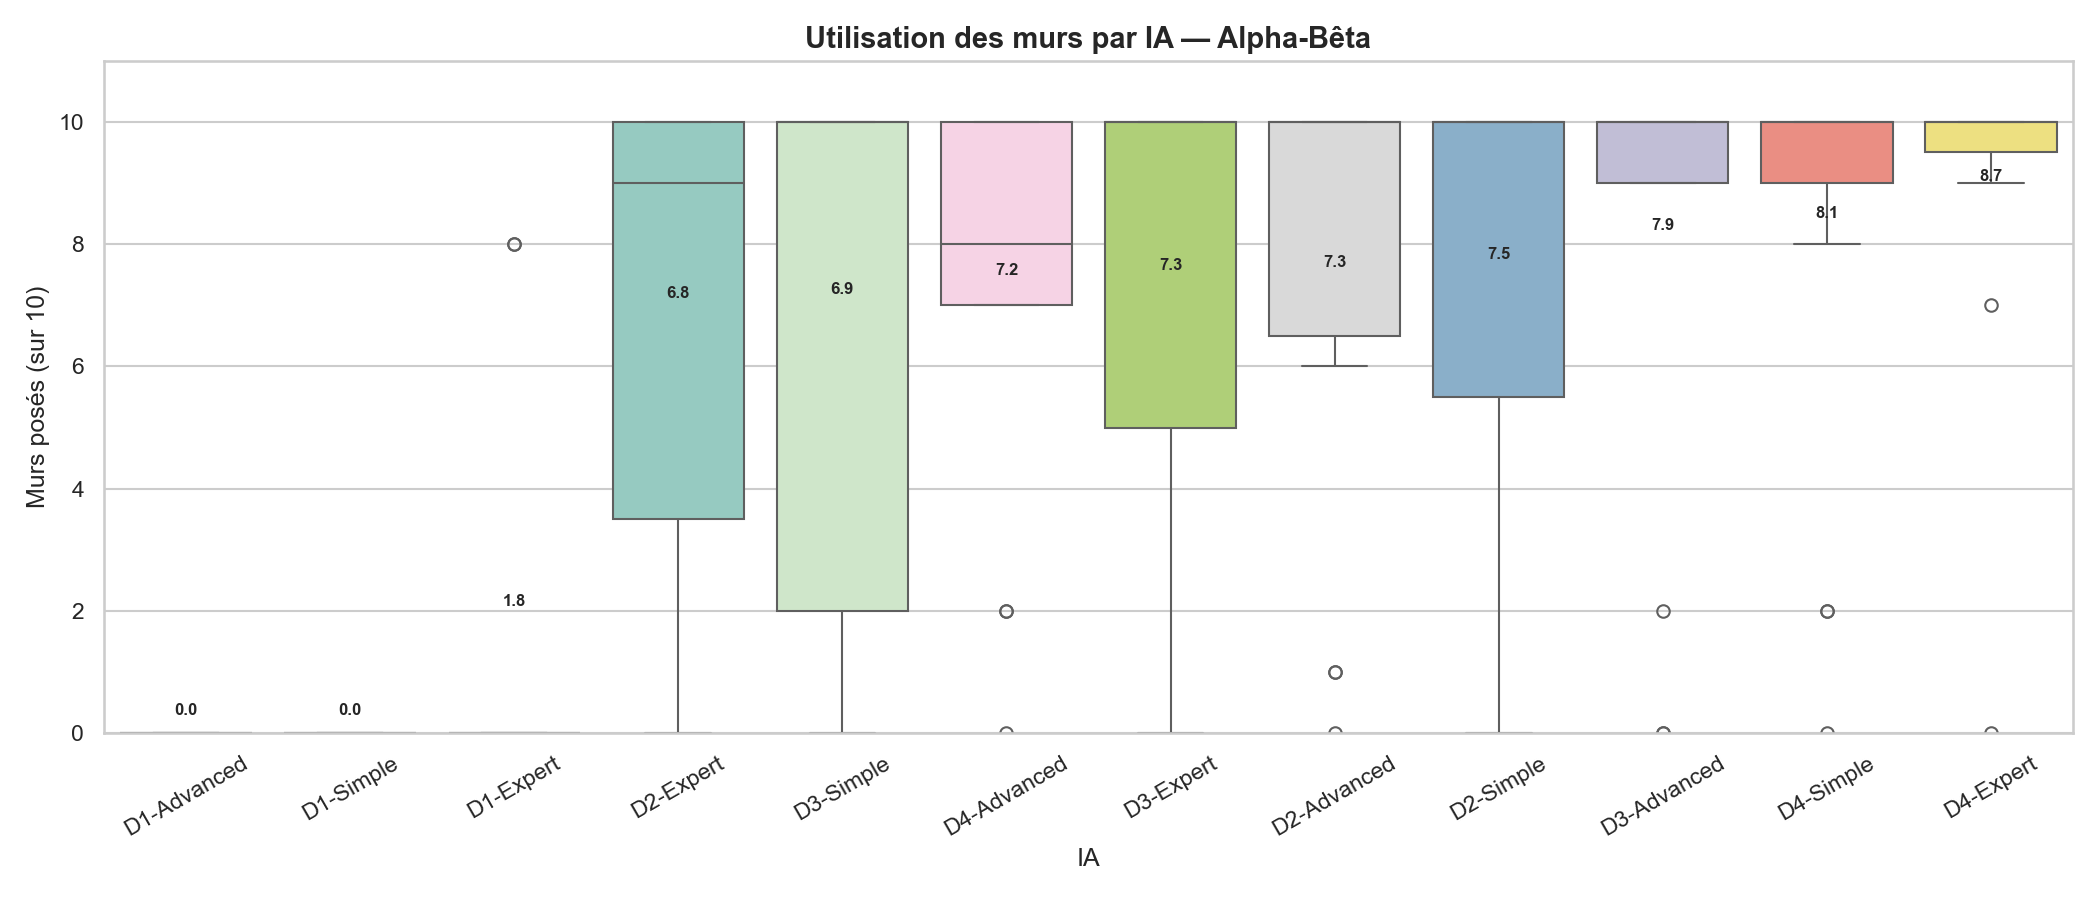
\includegraphics[width=0.85\textwidth]{../data/elagage/plots/murs_par_ia.png}
    \caption{Utilisation des murs --- Alpha-Bêta}
    \label{fig:murs-elagage}
\end{figure}

%------------------------------------------------------------------
\subsection{Comparaison Minimax pur vs Alpha-Bêta}

Le résultat le plus frappant : l'heuristique dominante s'inverse entre les deux tournois.

Avec le Minimax pur, l'expert domine (podium 100\% expert). Tous les n\oe{}uds sont explorés, donc ses 5 composantes évaluent chaque position de manière plus fine.

Avec l'Alpha-Bêta, c'est l'advanced qui prend le dessus (podium 100\% advanced). Ses 2 termes plus stables guident mieux l'élagage, alors que les scores dispersés de l'expert rendent les coupures moins fiables.

\begin{table}[H]
\centering
\caption{Comparaison des trois tournois}
\label{tab:comparaison}
\begin{tabular}{lccc}
\toprule
& \textbf{Minimax + random} & \textbf{Minimax pur} & \textbf{Alpha-Bêta} \\
\midrule
Durée totale & $\sim$2h & $\sim$2h & $\sim$20min \\
Heuristique dominante & expert & variée & advanced \\
Champion & D2-Expert & D4-Advanced & D4-Advanced \\
Tie-breaking & oui (0.2) & non & non \\
Hiérarchie profondeur & perturbée & partielle & respectée \\
\bottomrule
\end{tabular}
\end{table}

Le tournoi Alpha-Bêta est environ 6 fois plus rapide que les tournois Minimax. Ça colle avec la théorie : $O(b^{d/2})$ contre $O(b^d)$, soit avec $b \approx 12$, environ $12^2 = 144$ n\oe{}uds par niveau à D4 pour l'élagage contre $12^4 = 20\,736$ pour le Minimax pur.

Le Minimax sans tie-breaking et l'Alpha-Bêta ont le même champion : D4-Advanced. Le Minimax avec random donne un classement incohérent (D2-Expert premier). Le tie-breaking perturbe surtout les profondeurs élevées, où D4 évalue plus de coups et tombe plus souvent sur des égalités.

L'heuristique advanced domine avec l'Alpha-Bêta (podium 100\% advanced), mais pas avec le Minimax pur sans random où le classement est plus mélangé. Avec le Minimax pur, toutes les branches sont explorées, donc les différences entre heuristiques sont moins marquées.

%------------------------------------------------------------------
\section{Utilisation de l'IA générative}

\subsection{Outils utilisés}

On a utilisé deux outils, Claude et Gemini :
\begin{itemize}
    \item Claude via le navigateur, pour les discussions sur la conception, la réflexion sur l'architecture et les heuristiques, et l'aide au debug.
    \item Gemini via le navigateur, pour les recherches approfondies par rapport aux heuristiques, l'analyse des résultats obtenus, et la conception du rapport final.
\end{itemize}

\subsection{Ce qu'on en a fait}

\begin{itemize}
    \item Conception : discussion du choix des heuristiques, des critères d'évaluation, de la structure du tournoi.
    \item Code : l'IA a généré le squelette du moteur de jeu, une première version du minimax, et l'optimisation.
    \item Débogage : debug par rapport au blocage des IA. Claude a suggéré d'ajouter une pénalité, il a aussi suggéré l'ajout du tie-breaking pour rendre le jeu moins déterministe, mais on n'a pas gardé ce dernier.
    \item Rapport : aide à la structuration et à la rédaction, relecture et correction du document.
\end{itemize}

\subsection{Ce qui a marché et ce qui n'a pas marché}

L'IA accélère le développement, mais le code n'est pas toujours correct du premier coup. Exemple : la première version du filtrage des murs ne vérifiait pas que l'IA ne se bloquait pas elle-même. On ne l'a vu qu'en regardant une partie où l'IA posait un mur devant son propre pion.

L'anti-oscillation a demandé 3 ou 4 tentatives. Il fallait découpler la pénalité du score alpha-bêta, sinon l'élagage devenait incorrect. C'est le genre de subtilité que l'IA ne voit pas tout seul.

Le tie-breaking n'a pas énormément ajouté de valeur au projet : dans le tournoi, on se retrouvait avec une IA de profondeur 1 qui battait une IA de profondeur 4.

Chaque bout de code généré a été relu et testé. L'IA fait gagner du temps mais ne dispense pas de comprendre ce qu'on fait.

%------------------------------------------------------------------
\section{Difficultés rencontrées}

\subsection{Auto-blocage de l'IA}

Le bug le plus long à résoudre. L'IA posait des murs sans vérifier si ça rallongeait son propre chemin. Résultat : elle se construisait un labyrinthe autour d'elle-même. La correction est dans \texttt{moves\_optimization.py} : avant de garder un mur candidat, on simule sa pose et on vérifie avec un BFS que le gain de blocage dépasse le coût pour nous.

\subsection{Oscillation entre positions}

Les IA D1 faisaient des aller-retours entre deux cases. À profondeur 1, l'IA ne voit pas assez loin pour comprendre qu'elle tourne en rond. On a mis un historique de 6 positions et une pénalité de $-50$ pour les revisiter. Point important : cette pénalité ne s'applique qu'au choix final, pas dans la récursion alpha-bêta (sinon l'élagage est faussé).

\subsection{Temps de calcul à profondeur 3}

À D3, chaque coup prend environ 20 secondes. Pour un tournoi, c'est trop. Deux optimisations :
\begin{itemize}
    \item \texttt{\_fast\_copy} : copie manuelle du board (attribut par attribut) au lieu de \texttt{copy.deepcopy}. Environ 50 fois plus rapide, parce que nos attributs sont des types immutables.
    \item La réduction du facteur de branchement (de 72 à 10--15 coups) décrite en section 3.
\end{itemize}
Avec les deux, le tournoi tourne en 15 minutes environ.

\subsection{Gestion des sauts}

Plus compliqué que prévu. Il faut gérer le saut direct (par-dessus l'adversaire), le diagonal (quand un mur bloque derrière), le cas du bord (pas de saut hors de la grille), et les combinaisons. On a écrit des tests dédiés pour chaque cas.

\subsection{Pose de murs lors d'un match entre deux IA}
Au début du développement, quand une IA jouait contre une autre, elles ne posaient aucun mur. Les deux IA allaient tout droit, et ce pour toutes les profondeurs et heuristiques implémentées. Pour régler ce problème, on a dû ajouter des récompenses supplémentaires afin qu'une IA pose des murs.
\end{document}
